\chapter{Data and Monte-Carlo samples}
\section{Data sample}
The data used in this analysis was collected in pp collisions with centre-of-mass energy 2.76 TeV during the Run-1 of the LHC operation using the ATLAS detector. This was a dedicated 2013 run for a heavy-ion group with unusual for LHC low pie-up. The mean number of interactions per bunch crossing, as shown in Fig. \ref{ris:DataSampleMu} a) was lower, than 1. 

The this run \atlas collected 4.45 pb$^{-1}$ of data (Fig. \ref{ris:DataSampleMu} b)). However, not all of the data is applicable for a precise physics analysis, so the set of additional data quality (DQ) cuts was applied.  It uses an information about sub-detectors, that could be disabled during data-taking. These information is stored in so called Good Run List (GRL). Total luminosity, used in the analysis is 4.0 pb$^{-1}$. 

\begin{figure}[!b]
\begin{minipage}[h]{0.49\linewidth}
\center{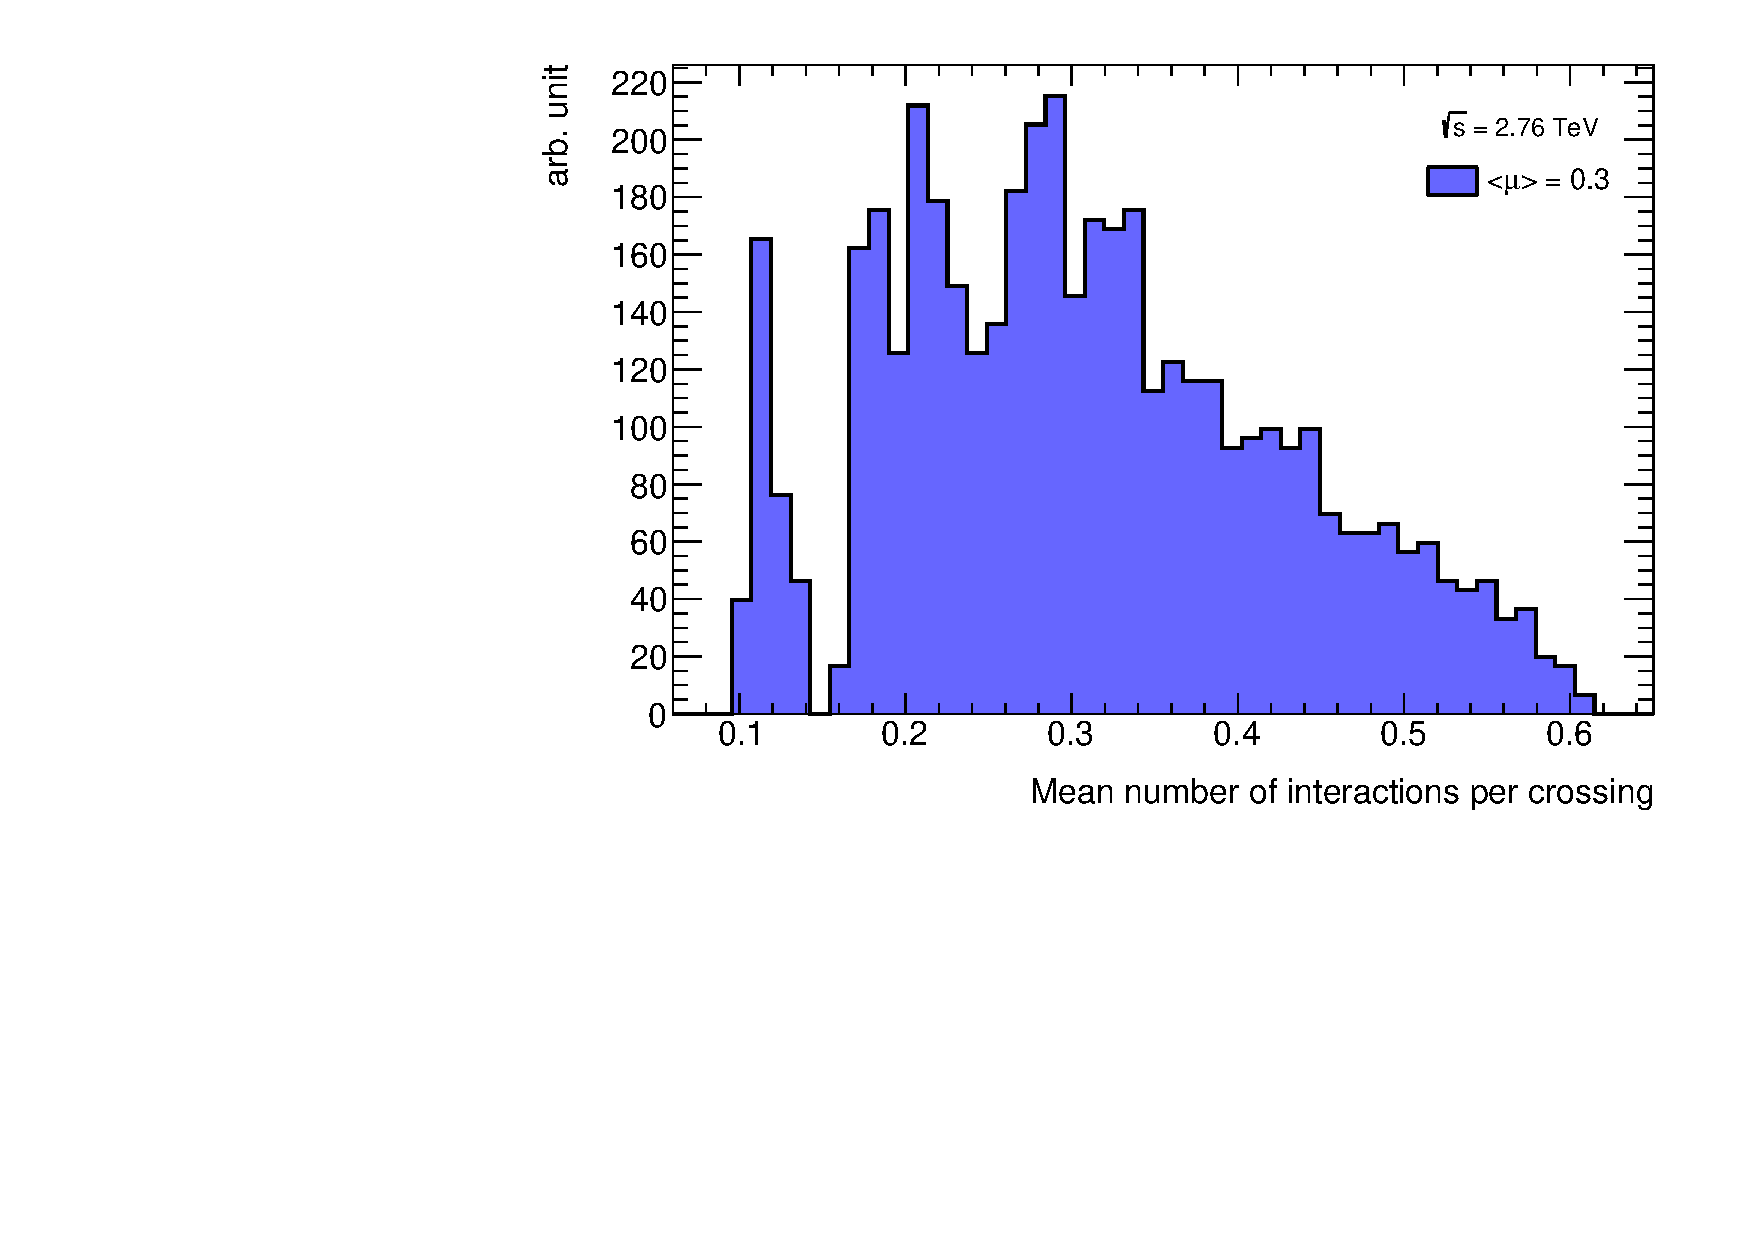
\includegraphics[width=1.\linewidth]{DataSample/mu.pdf}\\ a)}
\end{minipage}
\hfill
\begin{minipage}[h]{0.49\linewidth}
\center{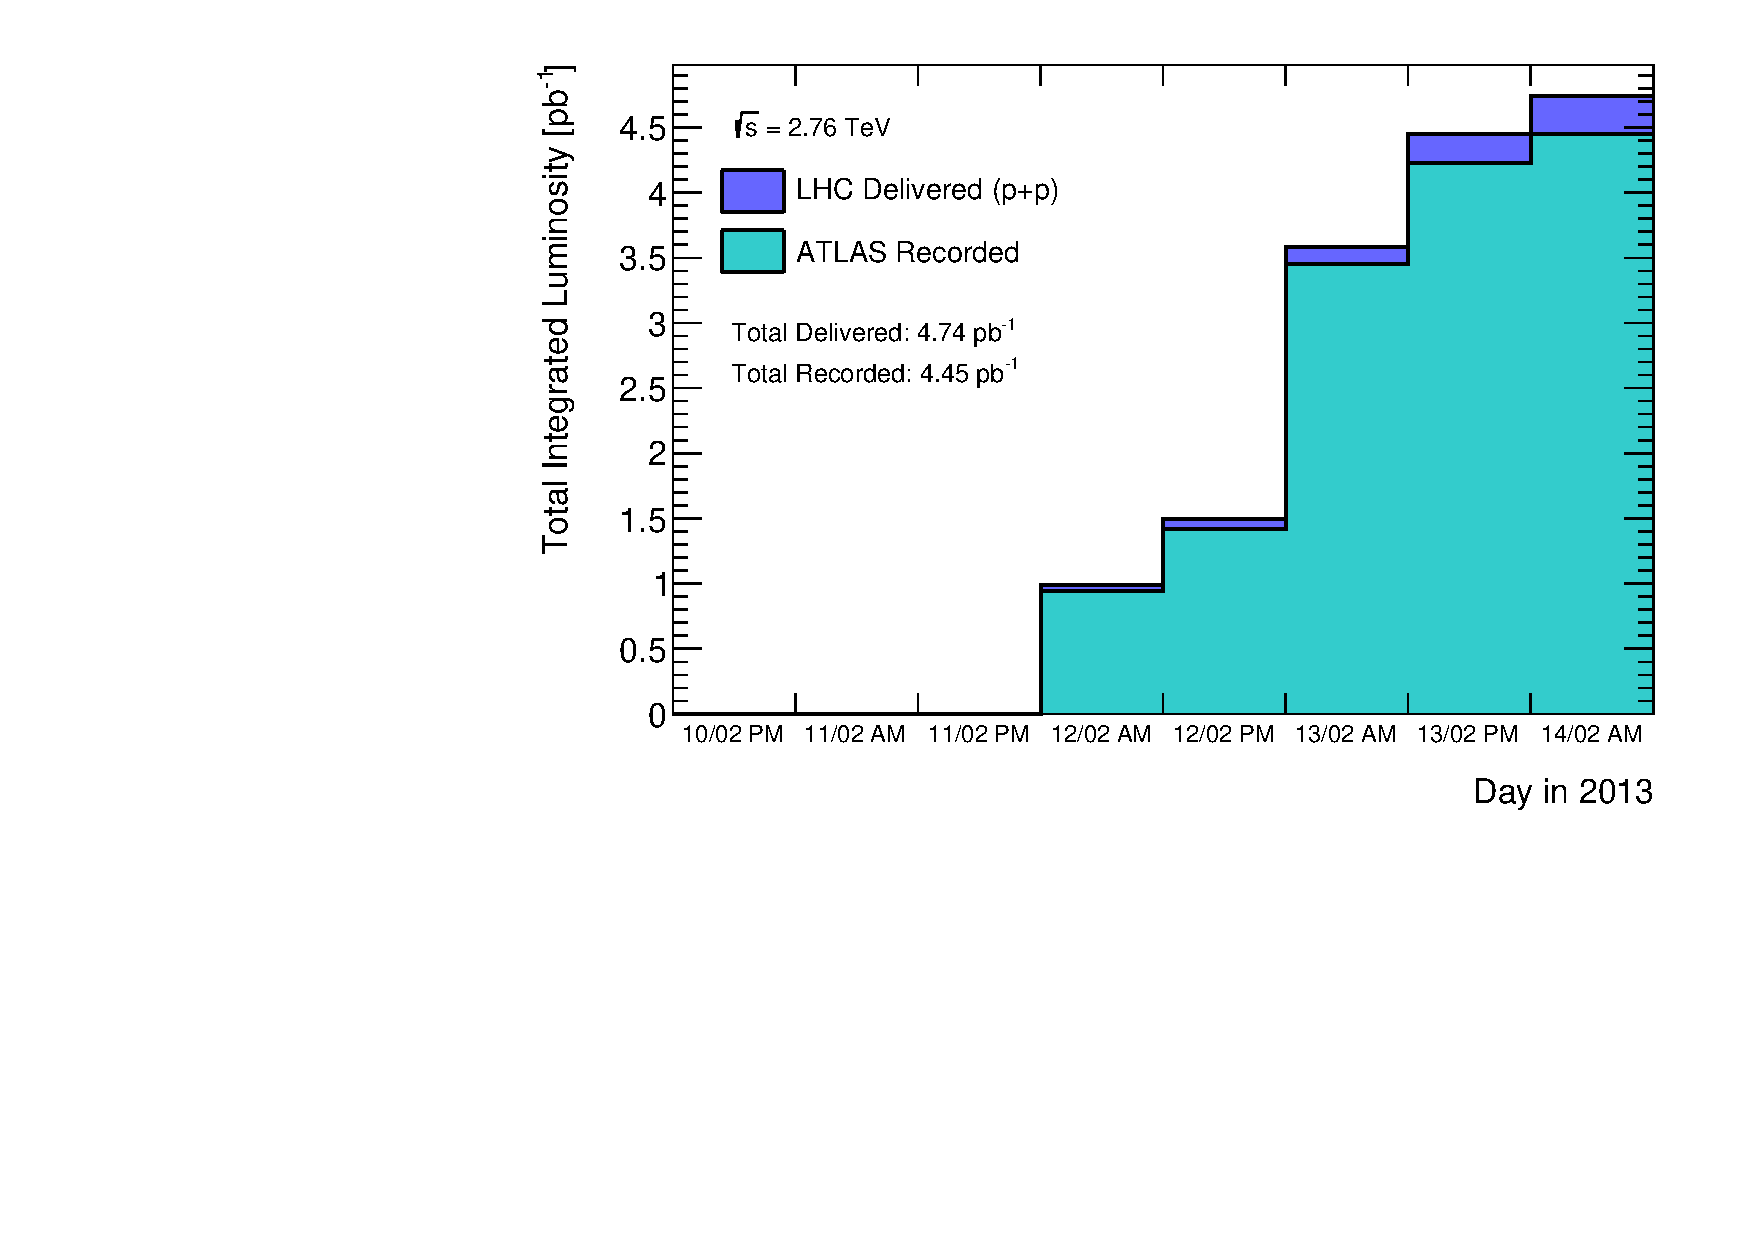
\includegraphics[width=1.\linewidth]{DataSample/lumi.pdf}\\ b)}
\end{minipage}
\caption{a) Mean number of interactions per bunch crossing. \\
b) Cumulative luminosity versus day delivered to (dark blue), and recorded by ATLAS (light blue) during stable beams and for pp collisions at 2.76 TeV centre-of-mass energy in 2013}
\label{ris:DataSampleMu}
\end{figure}

\section{Monte-Carlo samples}

The Monte-Carlo was used to simulate both signal and background processes. A summary of the MC samples used in analysis is given in Tab. \ref{tab:MCSamples}. The primary signals MC is generated using Powheg generator using CT10\cite{NewPartonD} PDFs interfaced with Pythi8 for parton showering using AU2\cite{ATL-PHYS-PUB-2012-003} tune. There is also additional signal MC sample for W-analyses, generated uisng Sherpa with CT10 PDFs. This sample is used for studies of the effect of matrix elements on final cross-section (see Chap. \ref{chap:Unc}).

The background sources are used to estimate fraction of the background events. The more detailed explanation of the background sources could be found in Chap. \ref{chap:Backgr}. The $W\to \tau\nu$ and $Z \to \tau\nu$ are generated similarly to signal MC with Powheg+Pythia8 generator with CT10 PDF and AU2 tune. Events with diboson decays are generated by Herwig with CTEQ6L1\cite{Pumplin2002} PDF set and using AUET2\cite{ATL-PHYS-PUB-2010-014} tune. The $t\bar{t}$ sample generated using Powheg generator interfaced with Pythia6. The additional $b\bar{b}$ and $c\bar{c}$ samples have been generated for QCD background determination and cross-check (Sec. \ref{sec:QCD}) and generated using Pythia8 with AU2 tune and CTEQ6L1 PDF set.



\begin{table}[!tb]
\caption{Monte-Carlo samples, used to simulate various signals and backgrounds.}
\label{tab:MCSamples}
\begin{center}
\begin{tabular}{l | c | c  }
Process & Generator & $N_{events}$ \\
\hline
& \multicolumn{2}{c}{Signal MC}\\
\hline
$W^{+} \to e\nu$ & Powheg+Pythia8 &  \\
$W^{-} \to e\nu$ & Powheg+Pythia8 & \\
$W^{+} \to \mu\nu$ & Powheg+Pythia8 &\\
$W^{-} \to \mu\nu$ & Powheg+Pythia8 &  \\
$Z \to ee$ & Powheg+Pythia8 &  \\
$Z \to \mu\mu$ & Powheg+Pythia8 &  \\
$W \to e\nu$ & Sherpa & \\
$W \to \mu\nu$ & Sherpa & \\
\hline 
\hline
& \multicolumn{2}{c}{Background MC} \\
\hline
$W^{+} \to \tau\nu$ & Powheg+Pythia8 &\\
$W^{-} \to \tau\nu$ & Powheg+Pythia8 & \\
$Z \to \tau\tau$ & Powheg+Pythia8 &  \\
$t \bar{t}$ & Powheg+Pythia6 &  \\
$WW$ & Herwig &   \\
$ZZ$ & Herwig &   \\
$WZ$ & Herwig &   \\
$b\bar{b}$ & Pythia8 & \\
$c\bar{c}$ & Pythia8 & \\
\hline
\end{tabular}
\end{center}
\end{table}